\chapter{Introduction}
\label{sec:Introduction}

I enjoy making music and I love listening to it. I was fascinated by one instrument in particular, the synthesiser. What I was fascinated by specifically was how every (at least hardware) synthesiser sounds a bit different; It is like they have their own little personality.

During the fourth semester, I went through a subject called "Programming in C++ I," and that is where the idea came up, the idea of making my own synthesiser. The result of this semester project was, although fairly unpolished and a bit of an incomplete, still a working "standalone" programme with a built-in MIDI support.

I didn't want to stop there. I wanted to extend this half-finished project into a fully-fledged bachelor's thesis that can be used in modern DAWs like FL Studio or Ableton Live as a VST plug-in. I was concerned that this could be just a copy of the existing synthesiser plug-ins already present on the market and that it would not be unique in any way. But in the end, I realised that this could still be a great opportunity to create a well documented, open-source synthesiser, along with a paper that could serve as a guide that would show you the process of making your own synth. In addition, I think one feature could be unique after all.

\subsection{Where I am right now}

Right now, my programme uses a few third-party libraries:
\begin{itemize}
    \item PortAudio, which opens up an audio stream that can be used to send data directly to the computer's speakers,
    \item libremidi, enabling MIDI support for connected MIDI devices, 
    \item ImGUI, simply to present the programme in some way, and
    \item SDL, specifically for polling the computer's keyboard input.
\end{itemize}

All of this will soon be substituted in favour of the JUCE framework. The reason why I originally chose these libraries is simply because of how large this framework is. I wanted to focus on the synthesiser instead and not spend hours learning JUCE right away; this would most likely prove not only to be challenging but also quite demotivating. This approach reduced additional, unneeded friction, while also keeping an independent architecture of the synth programme itself. Even though I will most likely run into some issues, overall, migrating the synth into the JUCE framework should actually end up being quite simple. After all, JUCE is used for building VST plug-ins, so it is equipped with all of these features already, all that is left is to substitute said libraries with them.

\subsection{Hardware inspired}

Synthesisers became really popular in the 1980s. A few years earlier, people and artists considered them a niche instrument, mostly because of their price point and incomprehensibility. But in the 1980s, they became a lot simpler, a lot more approachable, and eventually mainstream.

Back then, synthesisers were hardware. It was an electronic musical instrument with no moving parts that you could plug in and connect to another device (for example, another electronic instrument or a computer). Today, they are still used, but it is much more common to use a software synthesiser on your computer, which you can download or purchase. So-called soft synths, these simulate the real thing, the hardware variant.

The way in which most hardware synthesisers work can be described through its three crucial components: the oscillator, the filter, and the amplifier. The signal, which is interpreted as sound at the end, travels through these modules in that order. The oscillator is the module that generates this signal, it gets fed into the filter, which alters this signal in a certain way, this depends on what kind of filter we are using. For example, a low-pass filter would filter out certain high frequencies, making the final signal sound more mellow. A high-pass filter would filter out the low frequencies, eliminating the bass. This modified signal then reaches the amplifier, which makes the resulting sound louder and controls its volume.

The method described here is called "Subtractive synthesis" or "Wavetable synthesis" (I will get into the differences soon) and is one of the most common methods used today. A signal gets created in the oscillator, and that signal is "subtracted" through the filter, usually resulting in a warm, rich sound.

\begin{figure}
    \centering
    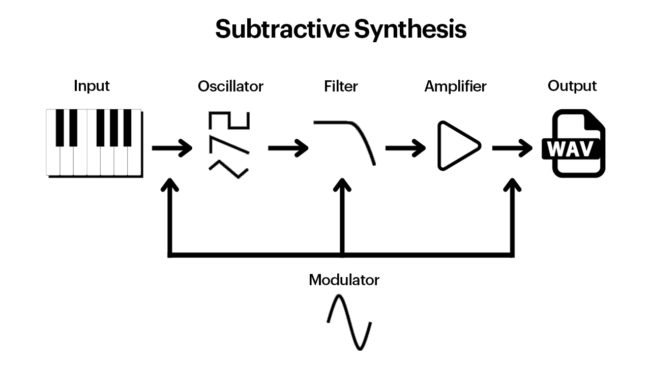
\includegraphics[width=0.8\linewidth]{Figures/subtractive-synthesis.jpg}
    \caption{Subtractive Synthesis.}
    \label{fig:placeholder}
\end{figure}

I looked at this diagram, and I thought I could approach it from the exact same perspective.

What does a hardware oscillator do? The ones used in synthesisers are voltage-controlled, so each key sends a certain amount of voltage, which then determines the outputted sound. The higher the voltage, the higher the circuit gets repeated, which equals a higher pitch. When substituting the circuit with a mathematical equation and voltage with direct frequency that a key sends, we can achieve pretty much the same result. The major difference is that the software variant can feel much more "synthetic," that is, compared to the "real deal." That's because the circuit on a hardware oscillator is sensitive to temperature, there is a slight pitch drift in real time - characteristics most people would probably never consider or notice, but musicians certainly do. Then again, if you want to achieve this "perfect" sound, then soft-synths are the way to go.

Since this circuit defines what its waveform will sound like, it will always only be that, full stop. In a programmed synth, you can substitute the equation with anything you like, this is the difference between traditional "Subtractive synthesis" and modern, software "Waveform synthesis" - storing any waveform you like and using that to generate sound? When you realise that these synths usually carry three oscillators, which you can combine at once, while also further filtering them; This is where Waveform synthesis becomes really impressive. Note that most basic waveforms can still be derived from the sawtooth waveform through additional circuits, but you cannot even get near the creativity you can achieve in the software variant.

\subsection{Next steps}

My current next step is to take the synth programme that I have written and strip it from the third-party libraries and embed it into the JUCE framework. After that, I would create a basic GUI that exposes the basic settings that the user should be able to manipulate with. For example, which oscillators should be active and what wavetables should they use, what filters to have active and what frequencies they should be filtering, and so on and so on.

After that, I would look into a few things that I considered "bugs" or overall parts that work, but could be improved upon. For example, in one part of the programme, I am using locking in threads, but I would like to utilise a thread-safe data structure (like a queue) instead.

There is one feature that I thought would be fairly cool to implement. For context, VST plug-ins are used in DAWs, digital audio workstations. A DAW is a piece of software that is used to create music. You can think of it as a video editing programme like DaVinci Resolve, for example, where there is a timeline, just with audio only. Onto this timeline, you put specific pieces of data that gets played on playback, they are called patterns in the case of MIDI signal, or samples in the case of pure audio, let us say, recorded on a microphone. You assign a specific VST plug-in (instrument) to each track to generate given MIDI notes using the said plug-in. This is the end goal of this programme, in the form of a VST plug-in that can be used to create music.

These DAWs obviously support looping; Having the ability to set a specific part of the timeline that should be repeated over and over. However, what if you don't want to use a whole DAW at the moment and want to just use the plug-in as a "standalone" application? Have fun with creating melodies without the need of starting a heavy application like FL Studio or Ableton Live. I miss this feature in the standalone variants of plug-ins, looping. You can only play the music in real time, and there is no way to save it to memory and let it loop repeatedly.

I would like to explore and, if possible, implement this in the standalone version of the app. There are many interesting problems that would require solving; like snapping recorded notes onto a grid based on a few parameters so that it matches the desired rhythm and is not "off." This is a feature that I am not yet quite certain of, and I will investigate it later to see if it is possible.

\endinput